% Test document for todofloats.sty: margin todonotes everywhere.
% Compile 3x with:  timeout 60 pdflatex -interaction=nonstopmode -output-directory=out test_todofloats.tex
% (check.sh does this and verifies the layout from the aux file.)
\documentclass[11pt,twocolumn]{article}
\usepackage[a4paper,margin=2.5cm,heightrounded=true,marginparwidth=59pt,marginparsep=10pt]{geometry}
\usepackage{hyperref}   % before algorithm, as in main.tex (acl.sty loads hyperref first)
\usepackage{caption}    % as acl.sty does; makes \captionof{algorithm} work with float.sty
\usepackage{lipsum}
\usepackage{graphicx}
\usepackage{booktabs}
\usepackage{algorithm}
\usepackage[noend]{algpseudocode}
\usepackage{tikz}
\usepackage{capt-of}
\usepackage{xcolor}
\definecolor{PGreen}{HTML}{CCD3CA}
\definecolor{PPink}{HTML}{EED3D9}

%%%%%%%%%%%%%%%%%%%%%%%%%%%%%%%%%%%%%%%%%%%%%%%%%%%%%%%%%%%%%%%%%%%%%%%%%
% TODONOTE CONFIGURATION (../../mytodonotes.sty on ../../todofloats.sty)
\usepackage[authors={timv=magenta!10},agents={claude,codex}]{mytodonotes} % [disable]
%%%%%%%%%%%%%%%%%%%%%%%%%%%%%%%%%%%%%%%%%%%%%%%%%%%%%%%%%%%%%%%%%%%%%%%%%
\usepackage[capitalise]{cleveref}   % as in main.tex (it re-patches \caption, needed for \captionof{algorithm})

\title{todofloats test document}
\author{check.sh}
\date{}

\begin{document}
\maketitle

\section{Two-column text, both columns}
Lorem ipsum dolor sit amet, consectetur adipiscing elit\timv{N1 first note, left column, normal text.} sed do
eiusmod tempor incididunt ut labore et dolore magna aliqua. Ut enim ad minim
veniam, quis nostrud exercitation ullamco laboris nisi ut aliquip ex ea commodo
consequat. Duis aute irure dolor in reprehenderit in voluptate velit esse cillum
dolore eu fugiat nulla pariatur.\claude{N2 a second author's note a few lines below N1.
\response{timv} And a response inside it.} Excepteur sint occaecat cupidatat non
proident, sunt in culpa qui officia deserunt mollit anim id est laborum.

\lipsum[2]

\subsection{Six notes close together (stacking)}
Line one has a note\timv{N3 stack 1 of 6.} here.
Line two has a note\timv{N4 stack 2 of 6, somewhat longer so that it takes three lines.} here.
Line three has a note\timv{N5 stack 3 of 6.} here.
Line four has a note\timv{N6 stack 4 of 6, again a longer one that wraps onto several lines in the margin.} here.
Line five has a note\timv{N7 stack 5 of 6.} here.
Line six has a note\timv{N8 stack 6 of 6.} here.

\lipsum[3]

\begin{figure}[t]
  \centering
  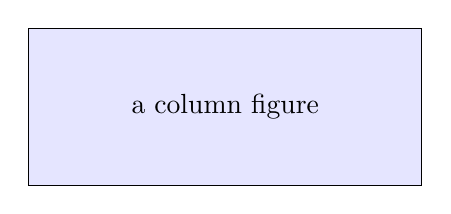
\begin{tikzpicture}
    \draw[fill=blue!10] (0,0) rectangle (5,2);
    \node at (2.5,1) {a column figure};
  \end{tikzpicture}
  \timv{N9 note inside a column figure float (outside the caption).}
  \caption{A column-width figure float.}
\end{figure}

\begin{table}[t]
  \centering
  \begin{tabular}{lrr}
    \toprule
    item & value\timv{N10 inside a tabular cell in a table float.} & unit \\
    \midrule
    a & 1 & kg \\
    b & 2\claude{N11 second note inside the same tabular.} & kg \\
    \bottomrule
  \end{tabular}
  \timv{N12 in the table float outside the tabular.}
  \caption{A column-width table float.}
\end{table}

\lipsum[4-5]

\begin{figure*}[t]
  \centering
  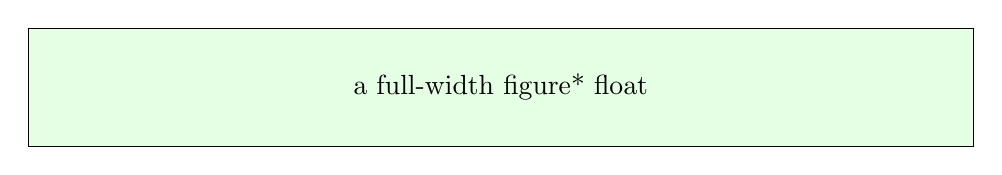
\begin{tikzpicture}
    \draw[fill=green!10] (0,0) rectangle (12,1.5);
    \node at (6,0.75) {a full-width figure* float};
  \end{tikzpicture}
  \timv{N13 inside a figure* full-width float.}
  \caption{A full-width figure.}
\end{figure*}

\section{More text and a minipage}
\lipsum[6]
This text is in the right column hopefully\timv{N14 note in the right column of two-column text.} and it
continues for a while so that the line breaks. \lipsum[7]

\noindent\begin{minipage}{\linewidth}
  A minipage with a margin note\timv{N15 inside a minipage.} in it; the note must not be lost.
  \lipsum[8]
\end{minipage}

\lipsum[9-11]

\begin{algorithm}[t]
  \caption{A floating algorithm in two-column mode.}
  \footnotesize
  \begin{algorithmic}[1]
    \Procedure{Demo}{$x$}
      \State $y \gets x$\timv{N16 on a State line in a floating algorithm (two-column).}
      \State $z \gets y + 1$ \Comment{a comment}\timv{N17 after a Comment.}
      \State \Return $z$
    \EndProcedure
  \end{algorithmic}
\end{algorithm}

\lipsum[12-14]

Near the bottom of a column: this line carries a long note\timv{N18 a long note near the bottom of the
page. It has to be lifted so that it does not run past the bottom of the text area. Lorem ipsum dolor
sit amet, consectetur adipiscing elit, sed do eiusmod tempor incididunt ut labore et dolore magna
aliqua. Ut enim ad minim veniam, quis nostrud exercitation ullamco laboris.} which must be shifted up.
And another one right after it\claude{N19 another long note right after N18, also near the bottom, that
must stack with N18 and be lifted with it. Duis aute irure dolor in reprehenderit in voluptate velit
esse cillum dolore eu fugiat nulla pariatur.} on the next line.

\onecolumn
\section{One-column part}
\lipsum[15]
In one-column mode notes always go to the right margin\timv{N20 one-column normal text.}, even when the
anchor is on the left half of the line.\claude{N21 one-column, second note close to N20.}

\begin{algorithm}[t]
  \caption{A floating algorithm in one-column mode.}
  \footnotesize
  \begin{algorithmic}[1]
    \Require a distribution $p$
    \Procedure{Sample}{$p$, $L$}
      \Repeat
        \State draw $z \sim p$\timv{N22 on a State line in a floating algorithm (one-column).}
        \State accept with probability $|z|/L$\claude{N23 on the next State line, stacks with N22.
        \response{timv} with a reply.}
      \Until{accepted} \Comment{acceptance probability $\le 1$}\timv{N24 after a Comment in a floating algorithm.}
      \State \Return $z$
    \EndProcedure
  \end{algorithmic}
\end{algorithm}

\lipsum[16]

\begin{figure}[t]
  \centering
  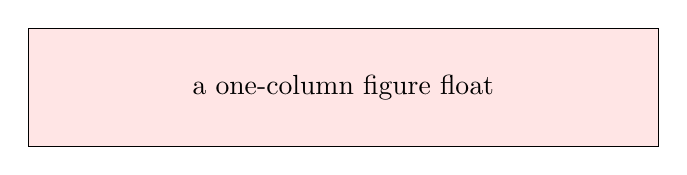
\begin{tikzpicture}
    \draw[fill=red!10] (0,0) rectangle (8,1.5);
    \node at (4,0.75) {a one-column figure float};
  \end{tikzpicture}
  \timv{N25 inside a figure float (one-column).}
  \caption{A one-column figure.}
\end{figure}

\begin{table}[t]
  \centering
  \begin{tabular}{lrr}
    \toprule
    item & value\timv{N26 inside a tabular cell in a table float (one-column).} & unit \\
    \midrule
    a & 1 & kg \\
    \bottomrule
  \end{tabular}
  \timv{N27 in the table float outside the tabular (one-column).}
  \caption{A one-column table.}
\end{table}

\noindent\begin{minipage}{\linewidth}
  A minipage in one-column mode with a note\timv{N28 inside a minipage (one-column).} in it.
  \lipsum[17]
\end{minipage}

\lipsum[18]

% non-floating algorithm block via \captionof (as in main.tex)
\noindent\begin{minipage}{\linewidth}
  \captionof{algorithm}{A non-floating captioned algorithm block.}
  \footnotesize
  \begin{algorithmic}[1]
    \State $a \gets 0$\timv{N29 in a captionof algorithm block (one-column).}
    \For{$i = 1, \ldots, n$}
      \State $a \gets a + i$ \Comment{running sum}\claude{N30 after a Comment in the captionof block.}
    \EndFor
    \State \Return $a$
  \end{algorithmic}
\end{minipage}

\lipsum[19-20]

Near the bottom of this one-column page: a long note\timv{N31 a long note near the bottom of a one-column
page, to be lifted so that it stays inside the text area. Lorem ipsum dolor sit amet, consectetur
adipiscing elit, sed do eiusmod tempor incididunt ut labore et dolore magna aliqua. Ut enim ad minim
veniam, quis nostrud exercitation ullamco laboris nisi ut aliquip ex ea commodo consequat.} anchored here.
And one more\claude{N32 the last note, stacked below N31 near the page bottom, also long enough to
matter. Duis aute irure dolor in reprehenderit in voluptate velit esse cillum dolore eu fugiat nulla
pariatur.} right after.

\lipsum[21]
A short inline note:\Timv{N33 a short inline note.}
\lipsum[22]

\clearpage
\section{Inline notes that break}\label{sec:inline-break}
\lipsum[23-25]
A long inline note starts here and has to continue on the next page.\Claude{\label{note:long-inline}I1 \textcolor{teal}{This whole
first part is teal, and the color has to survive the page break. \lipsum[26-27] The teal part ends here.}

A second paragraph in the note, with a display
\[ \sum_{n=1}^{N} n = \frac{N(N+1)}{2} \]
and a list:
\begin{enumerate}
\item first item, with a reference to \cref{sec:inline-break}
\item second item \lipsum[28]
\end{enumerate}
\lipsum[29-31]
\response{timv} A reply at the end of the long inline note, which refers to \cref{note:margin-cut} and \cref{note:long-inline,note:in-float}.}
Text right after the inline note. \lipsum[32]

\begin{figure}[t]
  \centering
  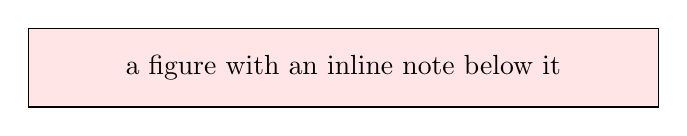
\begin{tikzpicture}
    \draw[fill=red!10] (0,0) rectangle (8,1);
    \node at (4,0.5) {a figure with an inline note below it};
  \end{tikzpicture}
  \Timv{\label{note:in-float}I2 an inline note inside a float: it cannot break, and it must not be lost.}
  \caption{A float with an inline note.}
\end{figure}

\begin{itemize}
\item A list item with an inline note:\Claude{I3 an inline note inside a list item, indented with the item text. \lipsum[33]}
and the item goes on.
\item Another item. In a box: \fbox{\Timv[inlinewidth=4cm]{I4 boxed.}}
\end{itemize}

\subsection{An Inline Note Right After a Heading}
\Timv{I5 directly after the heading; the heading must stay with the note.}
\lipsum[34]

\section{Margin notes that do not fit on the page}
\lipsum[35]
First anchor\timv{\label{note:margin-cut}M1 a margin note that is far too long for this page, so that it has to be cut and
continued in the margin of the next page. \textcolor{blue}{This blue passage is so long that it is still open
where the note is cut, and it must stay blue on the next page while the text of the document stays black.
\lipsum[36]} Black again. \lipsum[37] See \cref{sec:inline-break} and \cref{note:long-inline}.} in the text.
\lipsum[38]
Second anchor\claude{M2 a second long note on the same page, which has to keep its first lines next to its anchor.
\lipsum[39]
\response{timv} with a reply. \lipsum[40]} in the text.
\lipsum[41-44]
Third anchor on the following page\timv{M3 a note on the page that receives the continuation; it is stacked below it.} here.
\lipsum[45-47]

\twocolumn
\section{Two-column again}
\lipsum[48]
An inline note that breaks across columns.\Codex{I6 \lipsum[49-52]}
\lipsum[53]
Left column anchor\timv{M4 a long margin note in two-column mode. \lipsum[54-55]} and more text.
\lipsum[56-58]
The last note of the document overflows its page\claude{M5 this note is anchored on the last page and is too long for
it, so the document gets an extra page for the rest. \lipsum[59-61]} here.
\lipsum[62]
\end{document}
